\section{Experiments}
\label{sec:experiments}
\begin{table*}
\begin{center}
\setlength\tabcolsep{6pt} % default value: 6pt
\renewcommand{\arraystretch}{1.1}
\scalebox{0.8}{
\begin{tabular}{ l | c c c | c c c | c c c | c c c}
\toprule
\multicolumn{1}{c|}{\multirow{2}{*}{Methods}} & \multicolumn{3}{c|}{5\% Gaussians}  & \multicolumn{3}{c|}{10\% Gaussians}  & \multicolumn{3}{c|}{40\% Gaussians} & \multicolumn{3}{c}{70\% Gaussians} \\
\cline{2-13}
& PSNR$\uparrow$ & SSIM$\uparrow$ & LPIPS$\downarrow$ & PSNR$\uparrow$ & SSIM$\uparrow$ & LPIPS$\downarrow$ & PSNR$\uparrow$ & SSIM$\uparrow$ & LPIPS$\downarrow$ & PSNR$\uparrow$ & SSIM$\uparrow$ & LPIPS$\downarrow$ \\
\midrule
GGN~\cite{zhang2024gaussian} & N/A & N/A & N/A & N/A & N/A & N/A & 15.86 & 0.580 & 0.408 & 15.71 & 0.577 & 0.408 \\
AnySplat~\cite{jiang2025anysplat} & 8.08 & \second{0.229} & 0.593 & \second{10.37} & \second{0.363} & \second{0.513} & \second{19.66} & 0.677 & \second{0.248} & 21.85 & 0.723 & \second{0.177} \\
WorldMirror~\cite{liu2025worldmirror} & \second{8.09} & 0.220 & 0.632 & 10.20 & 0.349 & 0.552 & \second{19.66} & 0.692 & 0.277 & \second{22.11} & \second{0.744 }& 0.196 \\
% ZPressor~\cite{wang2025zpressor} +~\cite{fan2023lightgaussian} & xx.xx & x.xxx & x.xxx & xx.xx & x.xxx & x.xxx & xx.xx & x.xxx & x.xxx & xx.xx & x.xxx & x.xxx \\
% ZPressor~\cite{wang2025zpressor} +~\cite{HansonTuPUP3DGS} & xx.xx & x.xxx & x.xxx & xx.xx & x.xxx & x.xxx & xx.xx & x.xxx & x.xxx & xx.xx & x.xxx & x.xxx \\
% \jm{SPFSplat~\cite{huang2025no} + Opacity Prune} & 6.45 & 0.107 & 0.651 & 7.55 & 0.192 & 0.594 & 14.02 &0.586 & 0.341 & 20.79 & 0.778 & 0.197 \\
MVSplat~\cite{chen2024mvsplat} +~\cite{fan2023lightgaussian} & 5.82 & 0.053 & 0.717 & 6.41 & 0.085 & 0.696 & 8.71 & 0.224 & 0.598 & 9.26 & 0.245 & 0.581 \\
MVSplat~\cite{chen2024mvsplat} +~\cite{HansonTuPUP3DGS} & 5.86 & 0.051 & 0.699 & 6.66 & 0.096 & 0.678 & 9.00 & 0.232 & 0.590 & 9.26 & 0.245 & 0.580 \\
SPFSplat~\cite{huang2025no} +~\cite{fan2023lightgaussian} & 7.44 & 0.231 & 0.624 & 8.23 & 0.280 & 0.584 & 11.77 & 0.514 & 0.410 & 15.32 & 0.671 & 0.280 \\
SPFSplat~\cite{huang2025no} +~\cite{HansonTuPUP3DGS}& 6.48 & 0.167 & \second{0.589} & 7.61 & 0.256 & 0.536 & 12.01 & 0.522 & 0.378 & 16.72 & 0.697 & 0.257\\
\midrule
EcoSplat (Ours) & \best{24.72} & \best{0.822} & \best{0.183} & \best{25.00} & \best{0.831} & \best{0.171} & \best{25.11} & \best{0.835} & \best{0.164} & \best{25.00} & \best{0.832} & \best{0.166} \\
\bottomrule
\end{tabular}
}
\vspace{-0.2cm}
\caption{\textbf{Quantitative comparison of NVS under controlled numbers of primitives on the RE10K dataset~\cite{zhou2018stereo} with 24 input views.} 
\best{Red} and \second{Blue} indicate the best and second-best performances, respectively. `N/A' denotes that GGN~\cite{zhang2024gaussian} cannot achieve configurations with primitive counts below 15\% of the total number of pixel-aligned Gaussians due to its limited control over the primitive count.}
\label{table:primitive_ratio}
\vspace{-0.4cm}
\end{center}
\end{table*}

\begin{figure*}[t]
    \centering    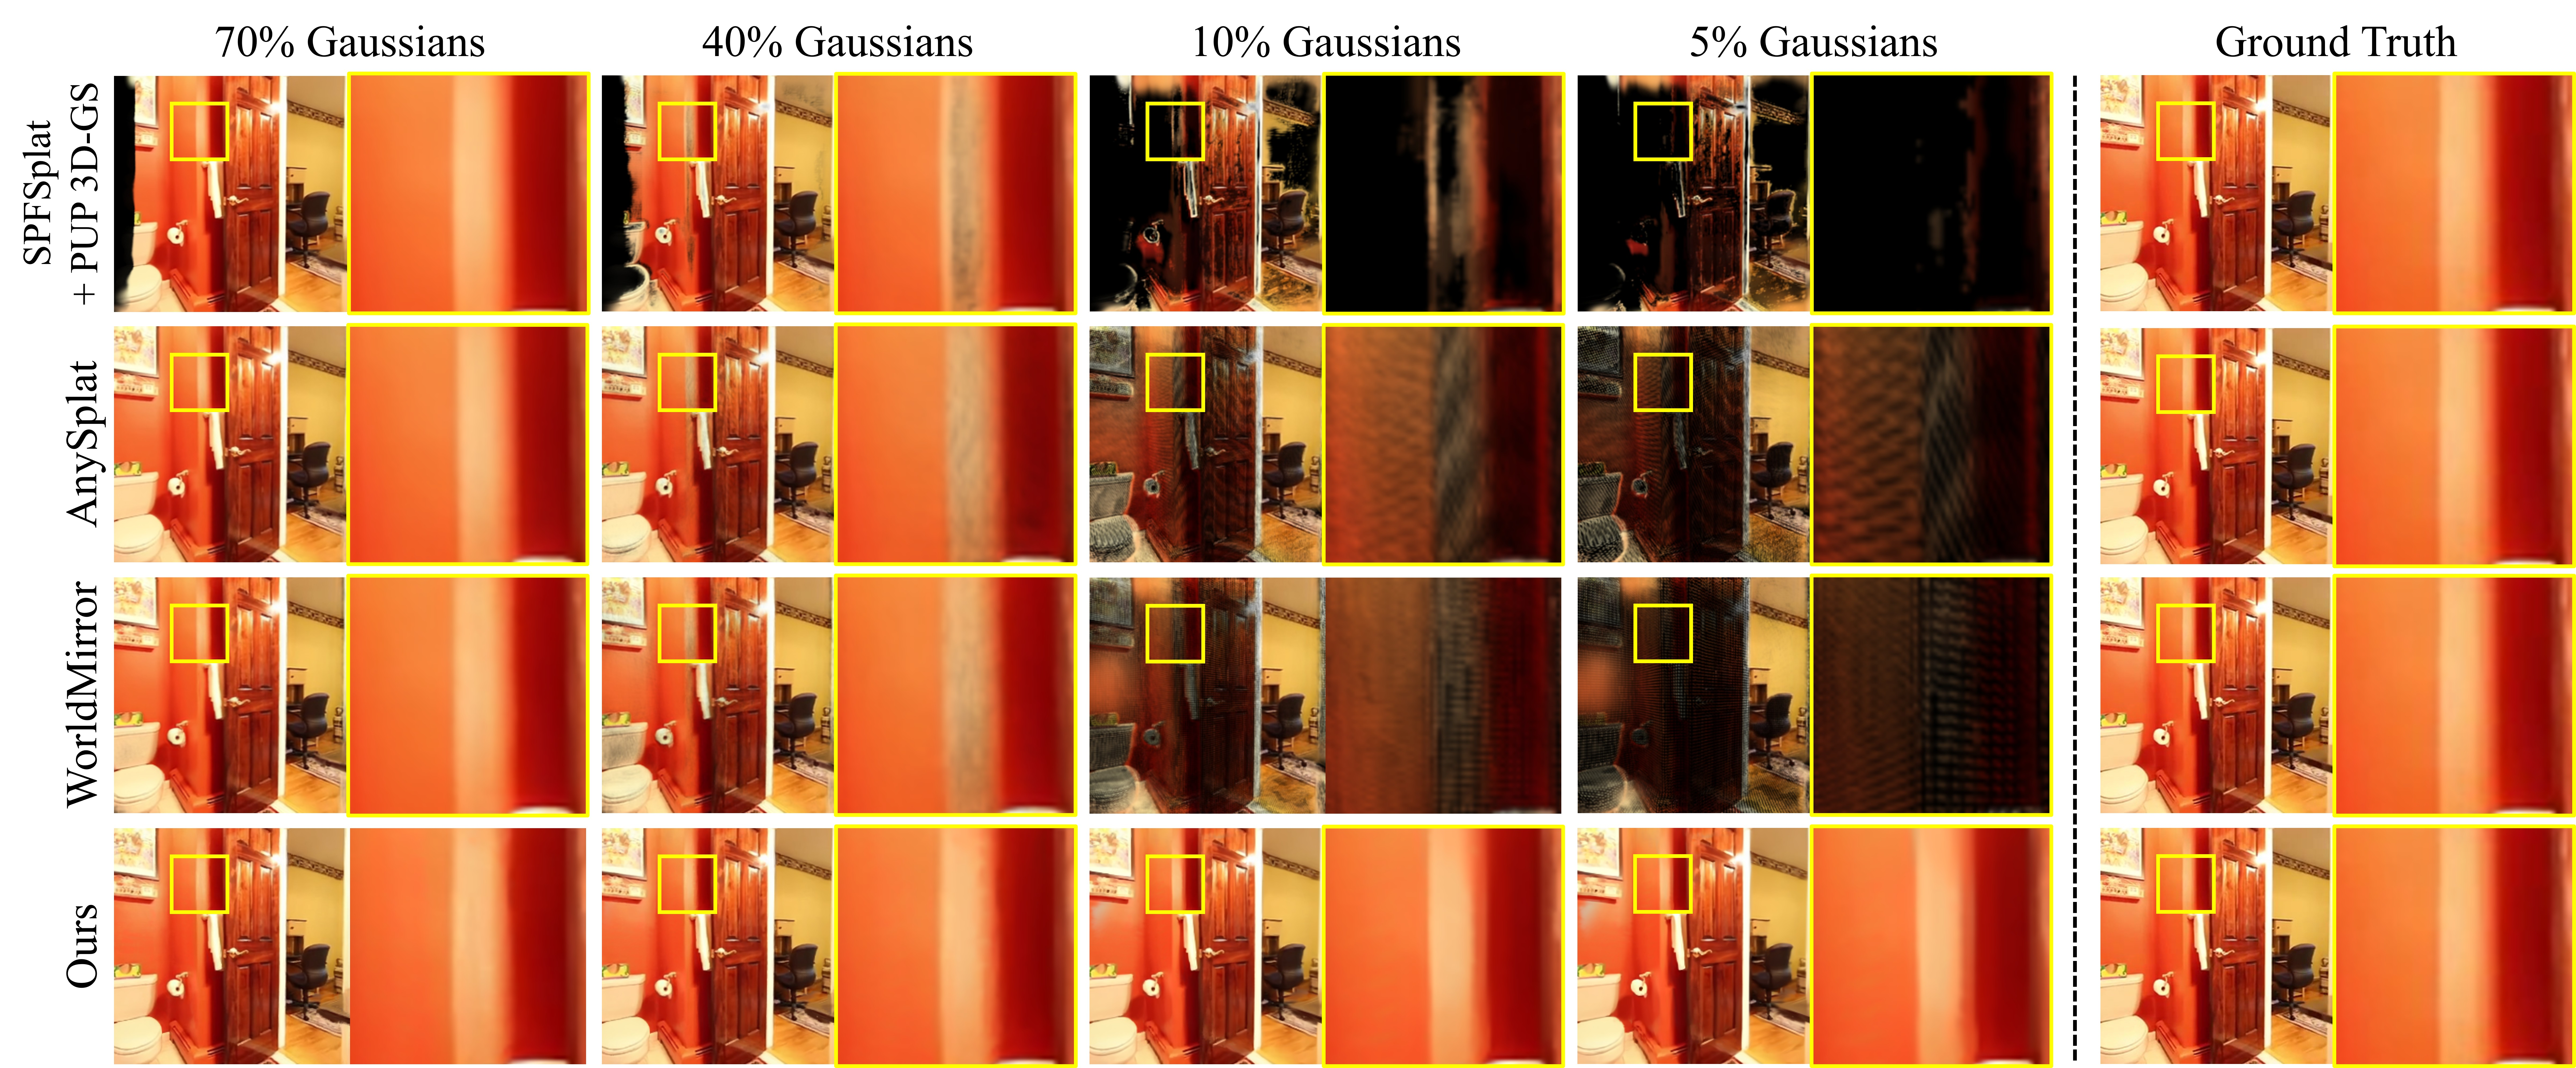
\includegraphics[width=0.98\linewidth,keepaspectratio]{figure/figure_3.jpg}
    \caption{\textbf{Visual comparison of NVS under controlled numbers of primitives on the RE10K dataset~\cite{zhou2018stereo} with 24 input views.}}
    \label{fig:qualitative_varying_K}
\end{figure*}


\noindent \textbf{Implementation Details.}
EcoSplat is implemented in PyTorch~\cite{Khvedchenya_Eugene_2019_PyTorch_Toolbelt} using the gsplat rasterization engine~\cite{ye2025gsplat}. Our training is conducted on 4 NVIDIA A100 GPUs (40GB each). Following prior works~\cite{huang2025no, ye2024no}, the ViT encoder/decoder and $F_\mu$ are initialized with pretrained weights from MASt3R~\cite{mast3r_eccv24}. For both PGT and IGF stages, we set the number of iterations to 200K. The number of decoder blocks $m$ is set to 4. For $\mathcal{L}_\text{io}$, we set $\lambda_\text{io}$ to 0.1. For PLGC, we set $\lambda_\text{decay}$ and $S$ to 0.05 and 1000, respectively. For Eq.~\ref{eq:high_frequency_score}, we set the side length of crop region $s$ to 64. For Eq.~\ref{eq:view_wise_impotance_factor}, we set $T$ to 0.2.

% \noindent \textbf{Implementation Details.} All details regarding our implementation are provided in the \textit{Supplementary}.

\noindent \textbf{Datasets.} 
We train our EcoSplat model on the large-scale {RealEstate10K (RE10K)} dataset~\cite{zhou2018stereo}, which contains over {10 million frames} collected from approximately {10K YouTube real estate videos}. To assess our model's rendering quality, we use the RE10K test split and the ACID dataset~\cite{infinite_nature_2020} for in-domain and cross-domain generalization, respectively. The ACID dataset~\cite{infinite_nature_2020} consists of thousands of aerial drone YouTube videos depicting diverse coastal and natural scenes. Following prior works~\cite{xu2025depthsplat, chen2024mvsplat, ye2024no, huang2025no}, our EcoSplat model is trained and evaluated at an image resolution of $256\times256$.

% We train our EcoSplat model on the large-scale {RealEstate10K (RE10K)} dataset~\cite{zhou2018stereo} and evaluate on both the RE10K test split and the ACID dataset~\cite{infinite_nature_2020}. More details of datasets are provided in the \textit{Supplementary}.

% which contains over {10 million frames} collected from approximately {10K YouTube real estate videos}. To assess our model's rendering quality, we use the RE10K test split and the ACID dataset~\cite{infinite_nature_2020} for in-domain and cross-domain generalization, respectively. The ACID dataset~\cite{infinite_nature_2020} consists of thousands of aerial drone YouTube videos depicting diverse coastal and natural scenes. Following prior works~\cite{xu2025depthsplat, chen2024mvsplat, ye2024no, huang2025no}, our EcoSplat model is trained and evaluated at an image resolution of $256\times256$.

\noindent \textbf{Evaluation Protocol.}  
We follow the evaluation protocol of NoPoSplat~\cite{ye2024no}. To evaluate model performance with a large number of input views, we first select challenging sequences from {NoPoSplat} characterized by large spatial gaps (0.05\%-0.3\% image overlap). We then densify these sparse sequences by randomly sampling intermediate views to meet our desired numbers of input views (e.g., 16, 20, 24 views). Following prior works~\cite{xu2025depthsplat,jiang2025anysplat, huang2025no, zhang2024gaussian, ye2024no}, we quantitatively evaluate NVS quality using Peak Signal-to-Noise Ratio (PSNR), Structural Similarity Index Measure (SSIM), and Learned Perceptual Image Patch Similarity (LPIPS)~\cite{zhang2018perceptual}. The final number of Gaussians is also reported as an additional metric to highlight EcoSplat's robustness when rendering for various numbers of primitives.

% To evaluate the effectiveness of our proposed {EcoSplat}, we conduct comprehensive comparisons against recent feed-forward 3DGS methods that enable controllable number of Gaussian Splats (GS) rendering, including {AnySplat}~\cite{jiang2025anysplat}, {LongLRM}~\cite{ziwen2025long}, and {GGN}~\cite{zhang2024gaussian}. Specifically, we vary the number of GS and assess the resulting reconstruction quality on the Re10K dataset~\cite{} using 16 input views.

% In addition, we compare rendering performance with leading feed-forward 3DGS baselines, including {DepthSplat}~\cite{xu2025depthsplat}, {NoPoSplat}~\cite{huang2025no}, {SPFSplat}~\cite{huang2025no}, {GCN}~\cite{zhang2024gaussian}, and {AnySplat}~\cite{jiang2025anysplat} under different input-view configurations (16, 24, and 32 views) on Re10K. To further assess generalization capability, we perform zero-shot dense reconstruction on the ACID dataset.

\begin{table*}
\begin{center}
\setlength\tabcolsep{6pt} % default value: 6pt
\renewcommand{\arraystretch}{1.1}
\scalebox{0.8}{
\begin{tabular}{ l | c c c c | c c c c | c c c c}
\toprule
\multicolumn{1}{c|}{\multirow{2}{*}{Methods}} & \multicolumn{4}{c|}{16 Views}  & \multicolumn{4}{c|}{20 Views}  & \multicolumn{4}{c}{24 Views} \\
\cline{2-13}
& PSNR$\uparrow$ & SSIM$\uparrow$ & LPIPS$\downarrow$ & \# GS$\downarrow$ & PSNR$\uparrow$ & SSIM$\uparrow$ & LPIPS$\downarrow$ & \# GS$\downarrow$ & PSNR$\uparrow$ & SSIM$\uparrow$ & LPIPS$\downarrow$ & \# GS$\downarrow$ \\
\midrule
MVSplat~\cite{chen2024mvsplat} & 14.88 & 0.463 & 0.435 & 1048K & 14.87 & 0.462 & 0.437 & 1310K & 14.86 & 0.461 & 0.440 & 1573K \\
DepthSplat~\cite{xu2025depthsplat} & 20.05 & 0.752 & 0.258 & 1048K & 19.53 & 0.733 & 0.274 & 1310K & 19.18 & 0.718 & 0.286 & 1573K \\
NoPoSplat~\cite{ye2024no} & 13.66 & 0.450 & 0.488 & 1048K & 13.47 & 0.441 & 0.496 & 1310K & 14.38 & 0.444 & 0.489 & 1573K \\
SPFSplat~\cite{huang2025no} & \second{25.09} & \best{0.841} & \best{0.141} & 1048K & \second{24.97} & \best{0.838} & \best{0.142} & 1310K & \second{24.74} & \second{0.832} & \best{0.145} & 1573K \\
GGN~\cite{zhang2024gaussian} & 15.82 & 0.578 & 0.409 & 425K & 15.81 & 0.578 & 0.408 & \second{472K} & 15.80 & 0.578 & 0.408 & \second{512K} \\
AnySplat~\cite{jiang2025anysplat} & 21.73 & 0.720 & 0.177 & 887K & 21.88 & 0.725 & 0.173 & 1078K & 21.90 & 0.724 & 0.173 & 1259K \\
WorldMirror~\cite{liu2025worldmirror} & 21.96 & 0.737 & 0.197 & 746K & 22.07 & 0.741 & 0.195 & 891K & 22.16 & 0.745 & 0.193 & 1020K \\ 
% ZPressor~\cite{wang2025zpressor} & - & - & - & 1048K & - & - & - & 1310K & - & - & - & 1573K \\
\midrule
Ours$_{5\%}$ & 24.77 & 0.823 & 0.182 &  \best{52K} & 24.78 & 0.825 & 0.181 &  \best{65K} & 24.72 & 0.822 & 0.183 &  \best{78K} \\
Ours$_{40\%}$ & \best{25.27} & \second{0.839} & \second{0.161} &  \second{419K} & \best{25.21} & \second{0.837} & \second{0.162} &  {524K} & \best{25.11} & \best{0.835} & \second{0.164} &  {629K} \\
\bottomrule
\end{tabular}
}
\vspace{-0.1cm}
\caption{\textbf{Quantitative comparison of NVS on the RE10K dataset~\cite{zhou2018stereo} under various input-view settings.} We evaluate all models with 16, 20, and 24 input views. `Ours$_{5\%}$' and `Ours$_{40\%}$' refer to our EcoSplat model constrained to 5\% and 40\% of the total pixel-aligned Gaussians, respectively. We provide the inference FPS for all baselines in the \textit{Supplementary}.}
\label{table:re10k_multi_view}
\vspace{-0.4cm}
\end{center}
\end{table*}

% \begin{figure*}[t]
%     \centering    \includegraphics[width=\linewidth,keepaspectratio]{figure/figure_multi_view.png}
%     \caption{\textbf{Visual comparisons of NVS with 24 input views:} (a) in-domain comparison on the RE10K dataset~\cite{zhou2018stereo}; (b) cross-domain generalization on the ACID dataset~\cite{infinite_nature_2020}. `Ours$_{5\%}$' and `Ours$_{40\%}$' refer to our EcoSplat model constrained to 5\% and 40\% of the total pixel-aligned primitives, respectively.}
%     \label{fig:qualitative_multi_view}
% \end{figure*}

\begin{table}
\begin{center}
\setlength\tabcolsep{6pt} % default value: 6pt
\renewcommand{\arraystretch}{1.1}
\scalebox{0.8}{
\begin{tabular}{ l | c c c c}
\toprule
\multicolumn{1}{c|}{Methods} & PSNR$\uparrow$ & SSIM$\uparrow$ & LPIPS$\downarrow$ & \# GS$\downarrow$\\
% \cline{2-13}
\midrule
MVSplat~\cite{chen2024mvsplat} & 18.09 & 0.500 & 0.379 & 1573K \\
DepthSplat~\cite{xu2025depthsplat} & 19.78 & 0.688 & 0.289 & 1573K \\
NoPoSplat~\cite{ye2024no} & 16.87 & 0.496 & 0.413 & 1573K \\
SPFSplat~\cite{huang2025no} & \best{24.40} & \best{0.720} & \best{0.222} & 1573K \\
GGN~\cite{zhang2024gaussian} & 18.06 & 0.553 & 0.389 & \second{475K} \\
AnySplat~\cite{jiang2025anysplat} & 21.96 & 0.619 & 0.258 & 1230K \\
WorldMirror~\cite{liu2025worldmirror} & 22.34 & 0.658 & 0.273 & 1141K \\
% ZPressor~\cite{wang2025zpressor} & - & - & - & - & - & - & - & - & - & - & - & - \\
\midrule
Ours$_{5\%}$ & 23.87 & 0.689 & 0.282 & \best{78K} \\
Ours$_{40\%}$ & \second{24.02} & \second{0.696} & \second{0.256} & 629K \\
\bottomrule
\end{tabular}
}
\caption{\textbf{Cross-dataset generalization with 24 input views.} We train all methods on the RE10K dataset~\cite{zhou2018stereo} and evaluate their zero-shot performance on the ACID dataset~\cite{infinite_nature_2020}. We provide results for 16 and 20 views in the \textit{Supplementary}.}
\label{table:acid_multi_view}
\vspace{-0.6cm}
\end{center}
\end{table}

\subsection{Comparison with State-of-the-Art Methods}
\noindent \textbf{NVS under Controlled Number of Primitives.}
Table~\ref{table:primitive_ratio} and Fig.~\ref{fig:qualitative_varying_K} present quantitative and qualitative comparisons of feed-forward 3DGS models under varying target 3D Gaussian counts, which are set to 5\%, 10\%, 40\%, and 70\% of the total pixel-aligned primitives ($NHW$). For this comparison, we use the RE10K dataset with 24 input views.
We compare our EcoSplat with representative efficient feed-forward 3DGS methods, such as GGN~\cite{zhang2024gaussian}, AnySplat~\cite{jiang2025anysplat}, and WorldMirror~\cite{liu2025worldmirror}. Since these methods lack \textit{explicit} control over the primitive counts at inference, we tune their relevant hyperparameters to \textit{indirectly} control the primitive counts, such as similarity thresholds for GGN~\cite{zhang2024gaussian} and voxel sizes for AnySplat~\cite{jiang2025anysplat} and WorldMirror~\cite{liu2025worldmirror}.
%In particular, we perform a binary search to identify the hyperparameter configurations that yield the desired number of primitives for each scene.
Furthermore, we compare our EcoSplat against the cascades of the SOTA pixel-aligned feed-forward 3DGS methods (SPFSplat~\cite{huang2025no} and MVSplat~\cite{chen2024mvsplat}) and the post-pruning methods~\cite{fan2023lightgaussian, HansonTuPUP3DGS}.
To preserve the feed-forward setting, we apply only the pruning step from~\cite{fan2023lightgaussian,HansonTuPUP3DGS} to the pixel-aligned Gaussians predicted by SPFSplat~\cite{huang2025no} and MVSplat~\cite{chen2024mvsplat}, with no additional optimization. As shown in Table~\ref{table:primitive_ratio}, existing methods experience substantial degradation as the number of allowed primitives decreases. Due to its limited algorithmic design, GGN~\cite{zhang2024gaussian} cannot reduce its primitive counts below a certain minimum threshold. Voxel-based approaches, such as AnySplat~\cite{jiang2025anysplat} and WorldMirror~\cite{liu2025worldmirror}, suffer from rendering artifacts at moderate pruning levels (e.g., $40\%$) and fail completely under aggressive pruning (e.g., $5\%$, $10\%$), as illustrated in Fig.~\ref{fig:qualitative_varying_K}.
%We show that combining pixel-aligned feed-forward models~\cite{huang2025no, chen2024mvsplat} with existing per-scene pruning techniques~\cite{fan2023lightgaussian, HansonTuPUP3DGS} is \jm{in}feasible.
Although LightGaussian~\cite{fan2023lightgaussian} and PUP 3D-GS~\cite{HansonTuPUP3DGS} perform reasonably well for zero-shot pruning on \textit{optimized}, per-scene 3DGS, they break down on feed-forward, pixel-aligned primitives. In these per-pixel representations, each Gaussian is tied to a single pixel, so pruning any primitive directly creates missing regions (Fig.~\ref{fig:qualitative_varying_K}).
In contrast, EcoSplat maintains high rendering fidelity over a wide range of primitive counts, with only marginal degradation even under aggressive reduction of primitives. These results highlight that EcoSplat shows the robustness and effectiveness of its explicit primitive-count control.

\noindent \textbf{NVS under Various Multi-view Settings.}
Table~\ref{table:re10k_multi_view} shows the NVS performance comparison of our EcoSplat against recent SOTA feed-forward 3DGS methods~\cite{xu2025depthsplat, ye2024no, huang2025no, zhang2024gaussian, ziwen2025long, jiang2025anysplat} across varying numbers of input views. For this comparison, we explicitly constrain our EcoSplat to extremely compact (5\%) and moderate (40\%) primitive ratios to demonstrate its robust performance.
As shown in Table~\ref{table:re10k_multi_view}, EcoSplat consistently achieves the best overall rendering qualities across all input-view configurations while using substantially fewer Gaussian primitives. Moreover, even with a primitive budget \textbf{$\sim$7$\times$ smaller} than the most compact baseline, GGN~\cite{zhang2024gaussian}, EcoSplat still achieves a \textbf{+9 dB} gain in PSNR and an LPIPS score that is \textbf{over 2$\times$ lower}. Compared to other efficient baselines such as AnySplat~\cite{jiang2025anysplat} and WorldMirror~\cite{liu2025worldmirror}, EcoSplat delivers \textbf{2.5-3.5 dB} higher PSNR while requiring \textbf{over 10$\times$ fewer primitives}. These results demonstrate that EcoSplat uniquely combines superior rendering quality with effective, explicit control over the primitive counts.

% As shown in Table~\ref{table:re10k_multi_view}, EcoSplat consistently achieves the best overall rendering quality across all input-view configurations while using substantially fewer Gaussian primitives. Specifically, EcoSplat attains SOTA performance even with only \textit{2.5$\times$ fewer primitives} compared to pixel-aligned methods such as SPFSplat~\cite{huang2025no}. Moreover, with a primitive budget that is approximately \textit{7-8$\times$ smaller} than the most compact feed-forward 3DGS approach, GGN~\cite{zhang2024gaussian}, EcoSplat still outperforms it by around \textit{+9 dB in PSNR} and achieves \textit{over 2$\times$ lower (better) LPIPS scores}. Compared to other efficient baselines such as AnySplat~\cite{jiang2025anysplat} and Long-LRM~\cite{ziwen2025long}, EcoSplat consistently delivers \textit{2.5-3.5 dB} higher PSNR while requiring \textit{over 10$\times$ fewer primitives}. These results demonstrate that EcoSplat not only enables effective control over the number of primitives but also achieves superior rendering quality compared to recent feed-forward 3DGS methods.

\noindent \textbf{Cross-Dataset Generalization NVS.}
% \input{table/acid_quantitative}
Table~\ref{table:acid_multi_view} shows the cross-dataset generalization performance of EcoSplat under multi-view settings, compared against recent SOTA feed-forward 3DGS methods~\cite{xu2025depthsplat, ye2024no, huang2025no, zhang2024gaussian, liu2025worldmirror, jiang2025anysplat}. For this comparison, we use the RE10K dataset~\cite{zhou2018stereo} for training and the ACID dataset~\cite{infinite_nature_2020} for evaluation.
EcoSplat consistently outperforms existing efficient feed-forward models and most of the pixel-aligned 3DGS methods except SPFSplat~\cite{huang2025no} in this setting. Note that EcoSplat underperforms SPFSplat with 0.38dB lower in PSNR, but uses substantially fewer primitives (only $40\%$). 


% \input{table/control_quantitative}
\subsection{Ablation Study}

% Table~\ref{tab:ablation} and Fig.~\ref{fig:ablation} present ablation results for the proposed EcoSplat components on the RE10K dataset~\cite{zhou2018stereo} under the 24-view setting with 5\% and 40\% primitive ratios.

\noindent \textbf{Training Strategy.}  
We validate our two-stage training strategy by ablating each stage, removing PGT and IGF to obtain the variants `w/o PGT' and `w/o IGF', respectively, as shown in Table~\ref{tab:ablation} and Fig.~\ref{fig:ablation}.
Under an extremely low primitive ratio (5\%), `w/o IGF' results in a drastic PSNR drop of over 18 dB and behaves similarly to the pixel-aligned feed-forward methods~\cite{chen2024mvsplat, huang2025no} in Table~\ref{table:primitive_ratio}.
Likewise, `w/o PGT' results in a 1.5 dB PSNR drop and visible rendering artifacts (Fig.~\ref{fig:ablation}), indicating the effectiveness of PGT.

\noindent \textbf{IGF Components.}
We vaildate the core components of the IGF stage, $\mathcal{L}_\text{io}$ and the PLGC strategy in Table~\ref{tab:ablation} and Fig.~\ref{fig:ablation}.
Without $\mathcal{L}_\text{io}$ (`w/o $\mathcal{L}_\text{io}$'), our model improperly allocates top-$K$ Gaussians relative to scene complexity, leading to under-reconstructed geometry and incomplete structural details (Fig.~\ref{fig:ablation}).
This results in significant degradation in both structural (PSNR, SSIM) and perceptual (LPIPS) metrics, especially under aggressive pruning (5\%).
Similarly, without the PLGC strategy (`w/o PLGC'), our model results in unstable optimization and fails to effectively adjust Gaussian parameters, leading to distorted outputs (Fig.~\ref{fig:ablation}).

\noindent \textbf{Importance-Aware Opacity Analysis.}
In Fig.~\ref{fig:opacity}, we visualize the opacity distributions predicted by EcoSplat for varying target primitive counts $K$ on a given scene. When $K$ is large (`70\% Gaussians', orange), the model retains a substantial proportion of high-opacity primitives that capture fine geometric and appearance details.
In contrast, when $K$ is reduced to 5\% (blue), EcoSplat effectively suppresses the opacities of low-importance primitives, pushing most of them toward the low-opacity region. Only a compact, highly informative subset maintains high opacity, corresponding to the most structurally and photometrically critical elements of the scene. This behavior illustrates that EcoSplat learns a robust importance ranking and dynamically adjusts Gaussian visibility according to the target primitive counts $K$.



% \begin{table}
% \begin{center}
% \setlength\tabcolsep{3pt} % default value: 6pt
% \renewcommand{\arraystretch}{1.1}
% \scalebox{0.7}{
% \begin{tabular}{ l | c c c | c c c }
% \toprule
% \multirow{2}{*}{Methods} & \multicolumn{3}{c|}{5\% Gaussians}  & \multicolumn{3}{c}{40\% Gaussians}  \\
% \cline{2-7}
% & PSNR$\uparrow$ & SSIM$\uparrow$ & LPIPS$\downarrow$ & PSNR$\uparrow$ & SSIM$\uparrow$ & LPIPS$\downarrow$ \\
% \midrule
% Deep attention & xx.xx & x.xxx & x.xxx & xx.xx & x.xxx & x.xxx \\
% Deep convolution & xx.xx & x.xxx & x.xxx & xx.xx & x.xxx & x.xxx \\
% % Shallow convolution (Ours) & 23.79 & 0.796 & 0.195 & xx.xx & x.xxx & x.xxx \\
% \midrule
% w/o PGT & xx.xx & x.xxx & x.xxx & xx.xx & x.xxx & x.xxx \\
% w/o IGF & 6.45 & 0.107 & 0.651 & 14.02 &0.586 & 0.341 \\
% w/o $\mathcal{L}_{io}$ & 20.58 & 0.724 & 0.289 & xx.xx & x.xxx & x.xxx \\
% % w/o $\mathcal{L}_{ac}$ & xx.xx & x.xxx & x.xxx & xx.xx & x.xxx & x.xxx \\
% w/o $\mathcal{L}_{progressive}$ & xx.xx & x.xxx & x.xxx & xx.xx & x.xxx & x.xxx \\
% Ours & 23.79 & 0.796 & 0.195 & 24.33 & 0.814 & 0.172 \\
% \end{tabular}
% }
% \vspace{-0.2cm}
% \caption{Ablation Study.}
% \label{table:nvidia_quantitative}
% \vspace{-0.4cm}
% \end{center}
% \end{table}


% \begin{table}[t]
% % \centering
% \setlength\tabcolsep{3pt}
% \renewcommand{\arraystretch}{1.1}
% \scalebox{0.78}{
% \begin{tabular}{@{}c@{}}
% % ---------- Subtable (a) ----------
% \begin{subtable}[t]{\linewidth}
% % \centering
% \begin{tabular}{l | c c c | c c c}
% \toprule
% \multicolumn{1}{c|}{\multirow{2}{*}{Loss Variant}} & \multicolumn{3}{c|}{5\% Gaussians} & \multicolumn{3}{c}{40\% Gaussians} \\
% \cline{2-7}
% & PSNR$\uparrow$ & SSIM$\uparrow$ & LPIPS$\downarrow$ & PSNR$\uparrow$ & SSIM$\uparrow$ & LPIPS$\downarrow$ \\
% \midrule
% w/o PGT & xx.xx & x.xxx & x.xxx & xx.xx & x.xxx & x.xxx \\
% w/o IGF & 6.45 & 0.107 & 0.651 & 14.02 &0.586 & 0.341 \\
% w/o $\mathcal{L}_{io}$ & 20.58 & 0.724 & 0.289 & 23.81 & 0.815 & 0.167 \\
% % w/o $\mathcal{L}_{ac}$ & xx.xx & x.xxx & x.xxx & xx.xx & x.xxx & x.xxx \\
% w/o $\mathcal{L}_{progressive}$ & 21.49 & 0.725 & 0.280 & 23.84 & 0.799 & 0.193 \\
% Ours & 23.79 & 0.796 & 0.195 & 25.11 & 0.835 & 0.164 \\
% \bottomrule
% \end{tabular}
% \captionsetup{font=small} % enlarge or adjust caption size
% \caption{.}
% \label{tab:ablation_loss}
% \end{subtable}
% \\[0.6em]
% % ---------- Subtable (b) ----------
% \begin{subtable}[t]{\linewidth}
% \centering
% \begin{tabular}{l | c c c | c c c}
% \toprule
% \multicolumn{1}{c|}{\multirow{2}{*}{Ablation Variant}} & \multicolumn{3}{c|}{5\% Gaussians} & \multicolumn{3}{c}{40\% Gaussians} \\
% \cline{2-7}
% & PSNR$\uparrow$ & SSIM$\uparrow$ & LPIPS$\downarrow$ & PSNR$\uparrow$ & SSIM$\uparrow$ & LPIPS$\downarrow$ \\
% \midrule
% Deep attention & 23.86 & 0.803 & 0.187 & 24.24 & 0.812 & 0.174 \\
% Deep convolution & 23.38 & 0.790 & 0.204 & 23.87 & 0.802 & 0.186  \\
% Ours & 23.79 & 0.796 & 0.195 & 25.11 & 0.835 & 0.164 \\
% \bottomrule
% \end{tabular}
% \captionsetup{font=small}
% \caption{.}
% \label{tab:ablation_architecture}
% \end{subtable}
% \end{tabular}
% }
% \vspace{-0.2cm}
% \caption{Ablation studies on the RE10K dataset. (a) compares loss configurations; (b) compares architectural variants.}
% \label{tab:ablation_full}
% \vspace{-0.3cm}
% \end{table}


\begin{table}[t]
\centering
\setlength\tabcolsep{3pt}
\renewcommand{\arraystretch}{1.1}
\scalebox{0.8}{
\begin{tabular}{l | c c c | c c c}
\toprule
\multicolumn{1}{c|}{\multirow{2}{*}{Variants}} & \multicolumn{3}{c|}{5\% Gaussians} & \multicolumn{3}{c}{40\% Gaussians} \\
\cline{2-7}
& PSNR$\uparrow$ & SSIM$\uparrow$ & LPIPS$\downarrow$ & PSNR$\uparrow$ & SSIM$\uparrow$ & LPIPS$\downarrow$ \\
\midrule
w/o PGT & 22.93 & 0.778 & 0.221 & 23.70 & 0.806 & 0.184 \\
w/o IGF & 6.45 & 0.107 & 0.651 & 14.02 &0.586 & 0.341 \\
w/o $\mathcal{L}_\text{io}$ & 20.58 & 0.724 & 0.289 & 23.81 & 0.815 & 0.167 \\
% w/o $\mathcal{L}_{ac}$ & xx.xx & x.xxx & x.xxx & xx.xx & x.xxx & x.xxx \\
w/o PLGC & 21.49 & 0.725 & 0.280 & 23.84 & 0.799 & 0.193 \\
\textbf{Ours} & 24.72 & 0.822 & 0.183 & 25.11 & 0.835 & 0.164 \\
\bottomrule
\end{tabular}
}
\vspace{-0.15cm}
\caption{\textbf{Ablation study on RE10K~\cite{zhou2018stereo} with 24 input views.}}
\label{tab:ablation}
\vspace{-0.25cm}
\end{table}



\begin{figure}[t]
    \centering    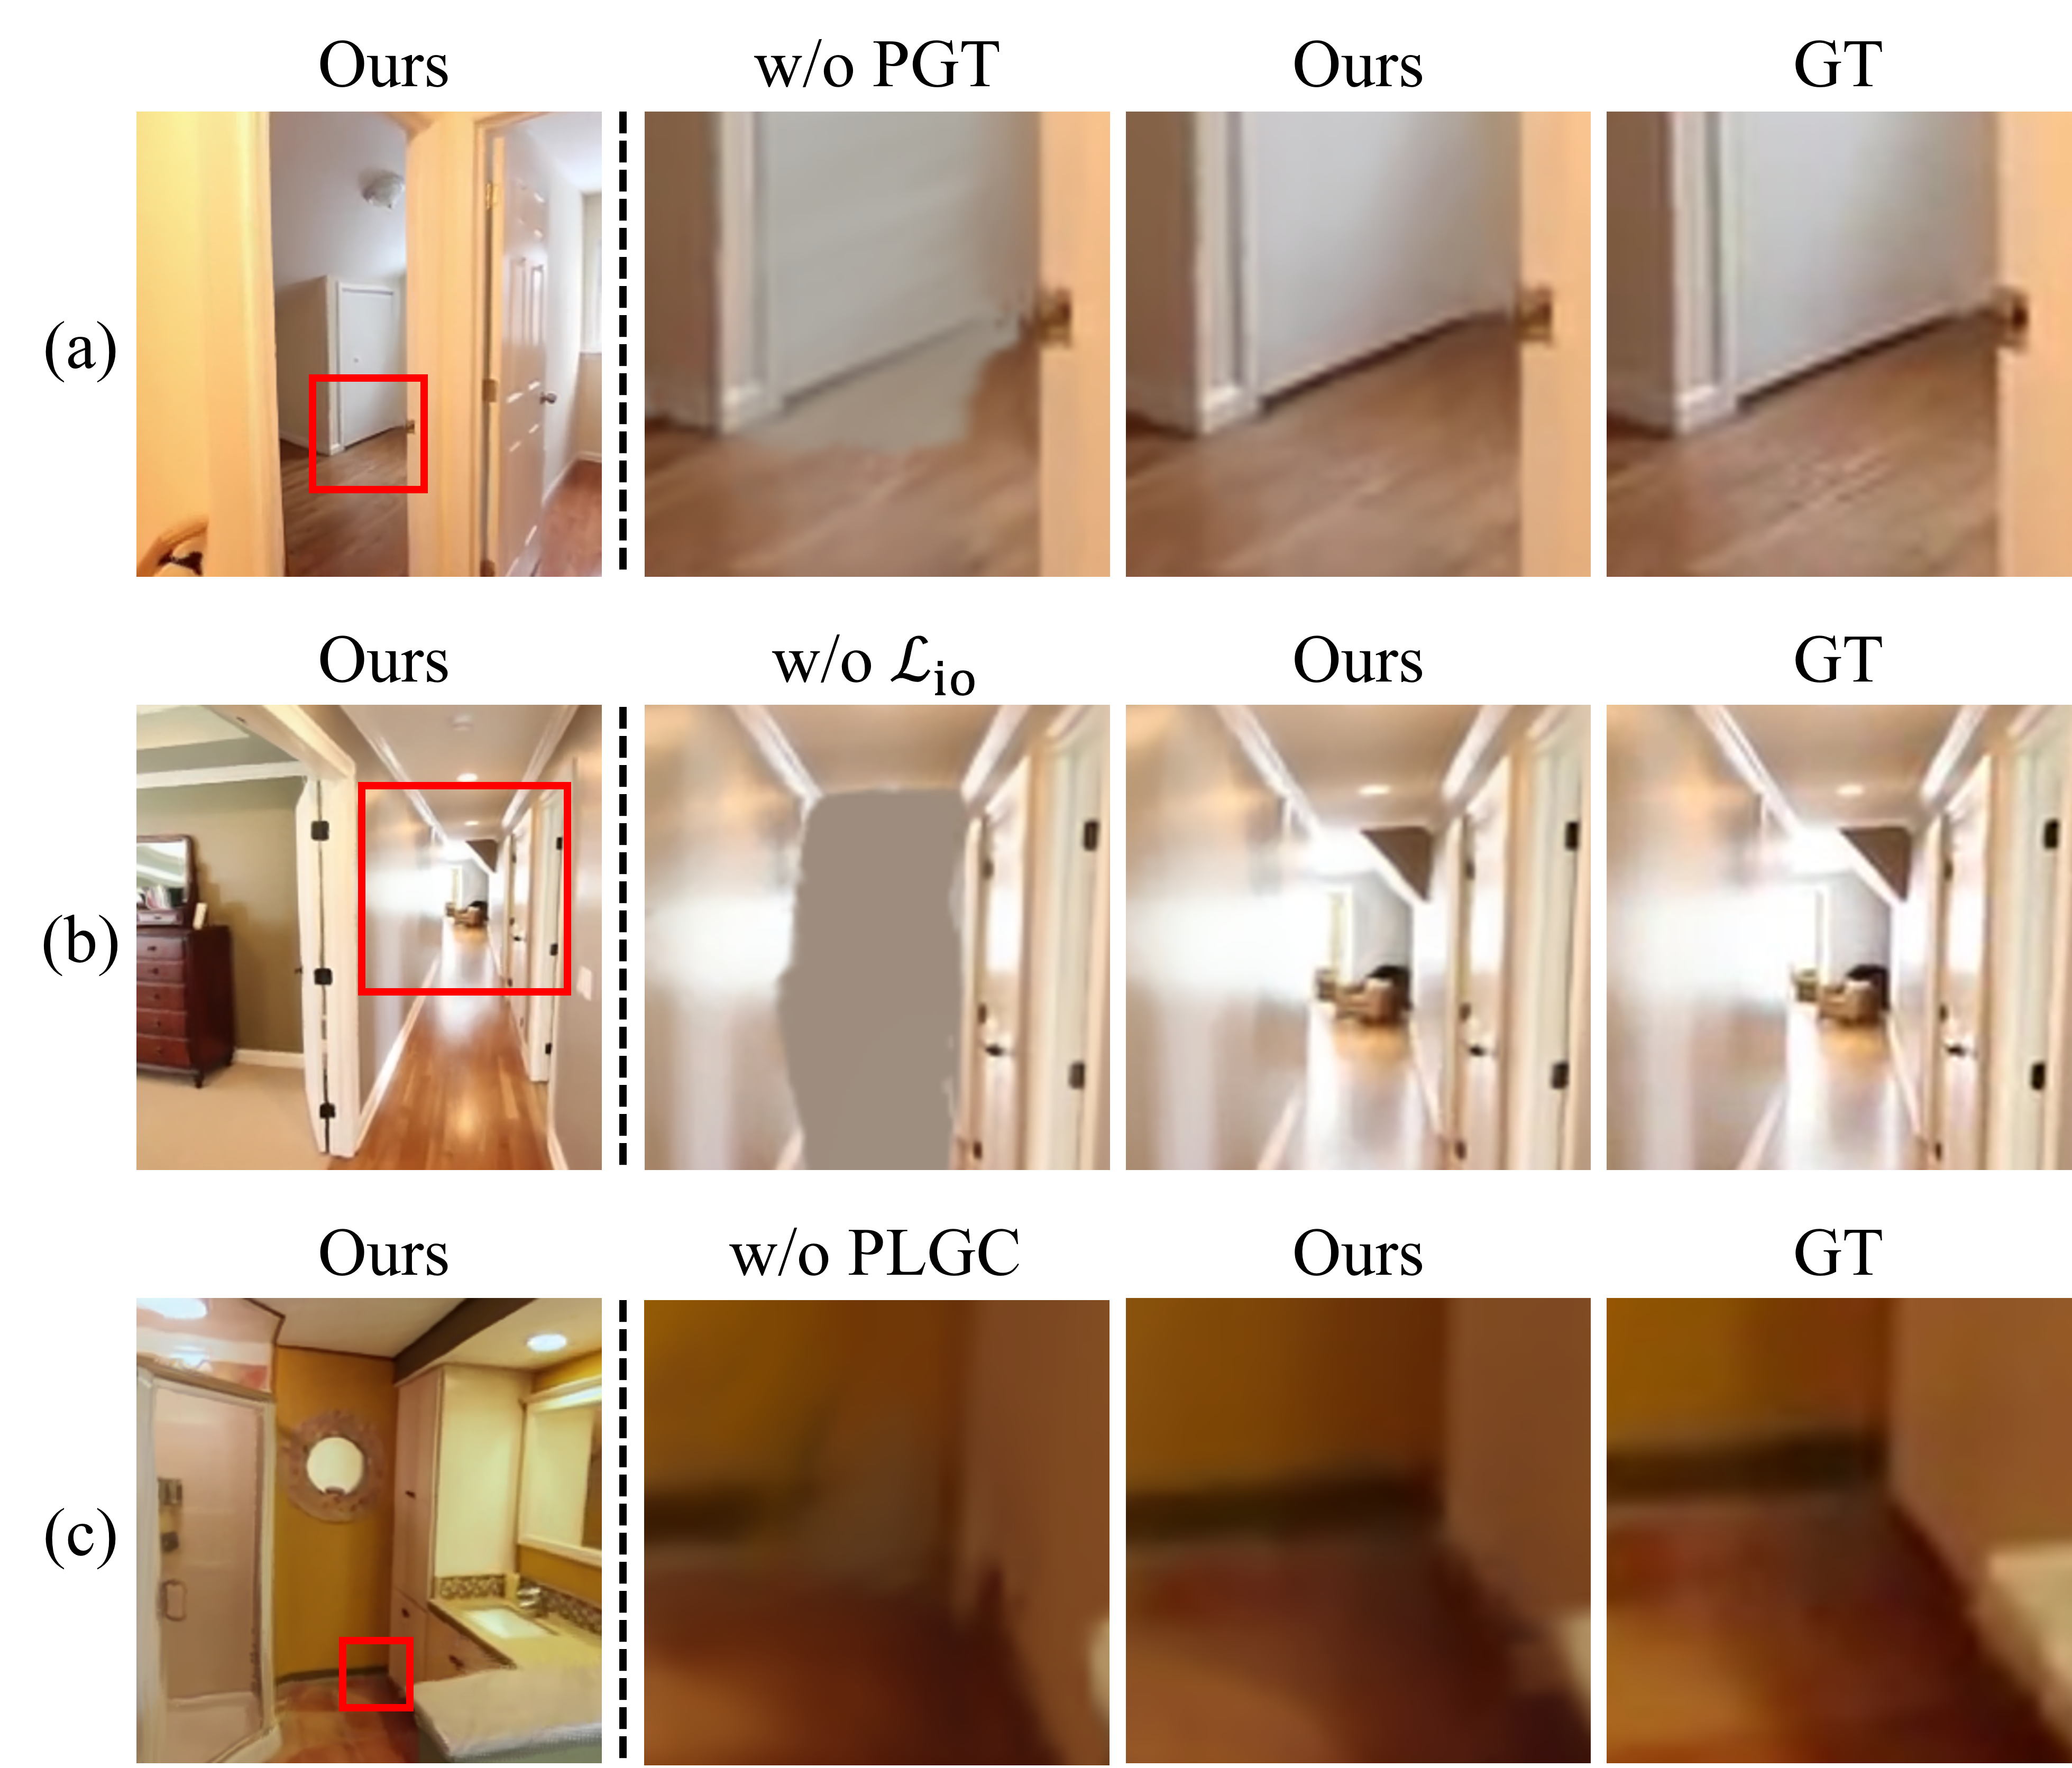
\includegraphics[scale=0.24]{figure/figure_ablation.png}
    \vspace{-0.2cm}
    \caption{\textbf{Visual results of ablation study:} (a) the PGT stage; (b) the importance-aware opacity loss; and (c) the PLGC strategy.}
    \label{fig:ablation}
\end{figure}

\begin{figure}[t]
    \centering    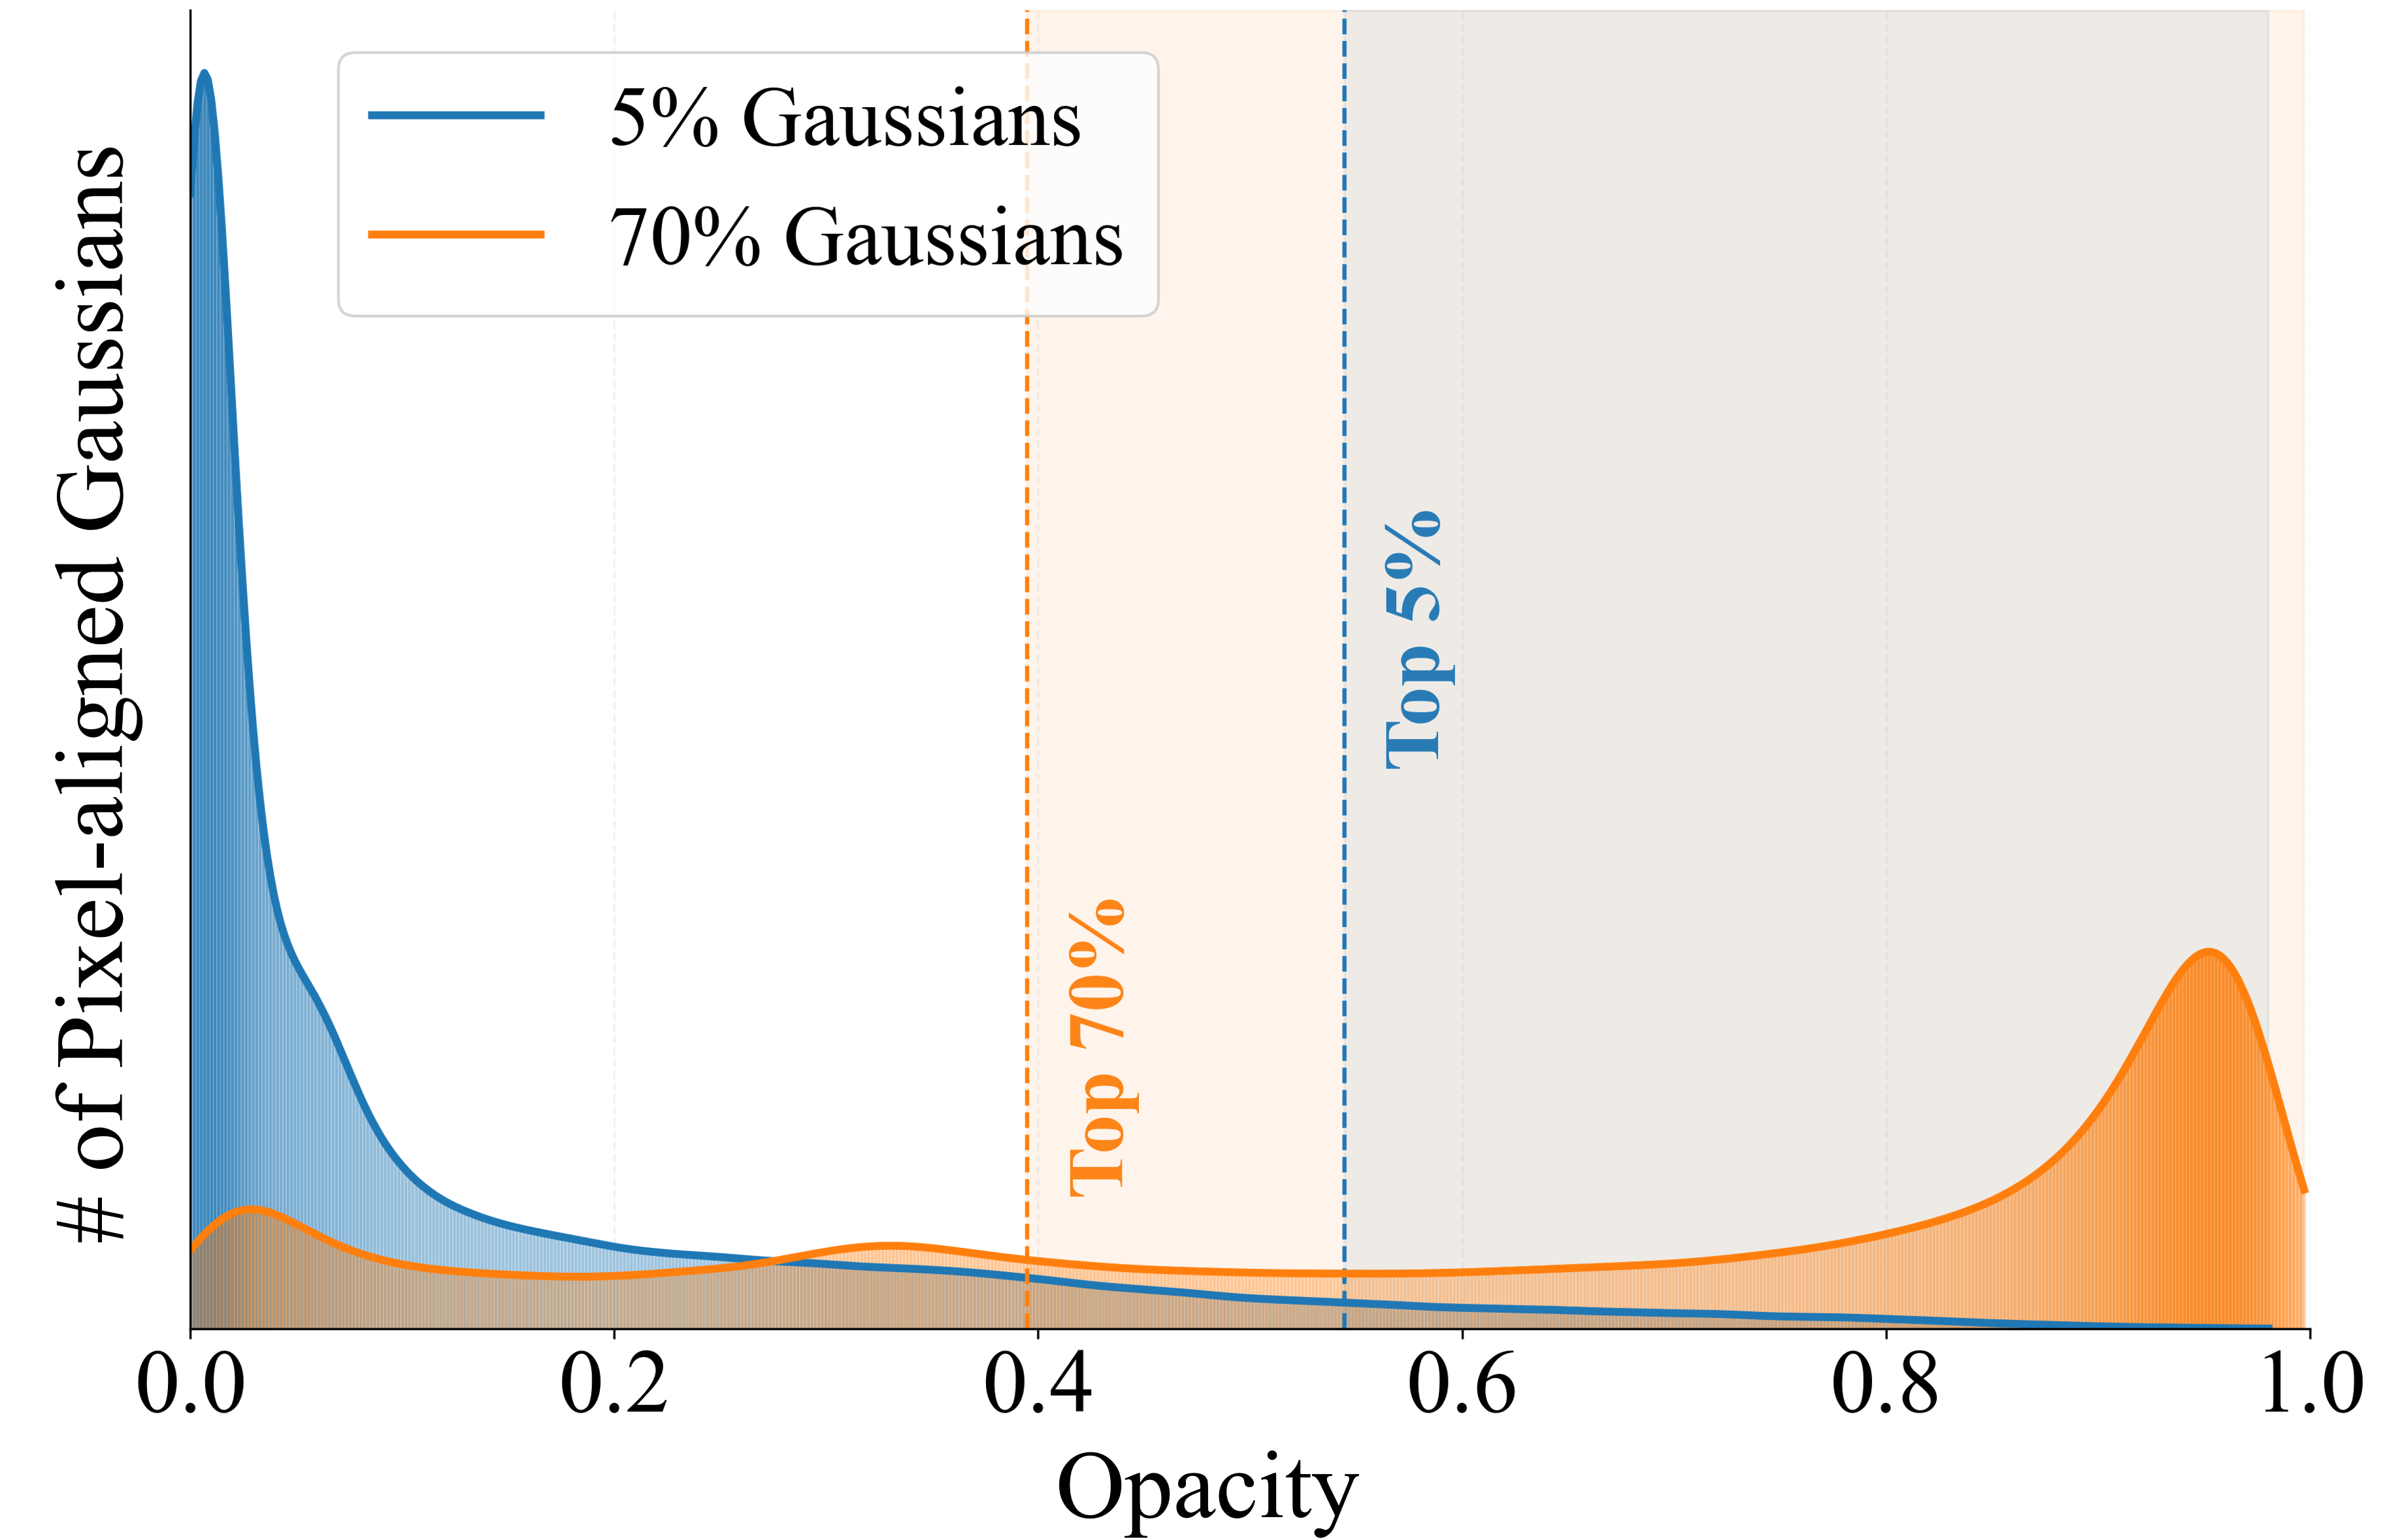
\includegraphics[scale=0.22]{figure/figure_5.png}
    \vspace{-0.3cm}
    \caption{\textbf{Opacity distributions of pixel-aligned Gaussians across target primitive counts $K$.} The blue and orange curves show the distributions when the target primitive count is set to 5\% and 70\% of the total number of pixel-aligned Gaussians, respectively. EcoSplat adaptively predicts Gaussian opacities based on the primitive budget and selects the top-$K$ Gaussians.}
    \label{fig:opacity}
\end{figure}
